\section{What traits do you share with your mother and father?}
I'm looking at physical traits first.
There are times when I look in the mirror and catch a glimpse of my mother's face.
It can be a smile or some other facial expression.
However growing up I thought I looked more like my father.
While I'm not tall I have a large bone structure, large hands and feet.
That was likely from my father's gene pool.
My blonde hair and blue eyes were likely from the Hess gene pool as well.
The following two pictures let you decide who I look like.
\begin{figure}
\centering
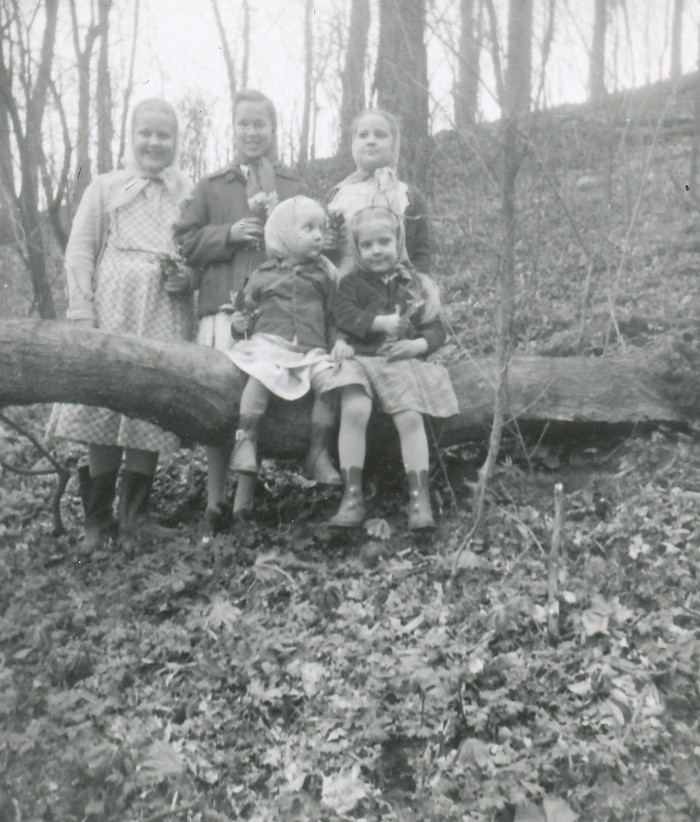
\includegraphics[height=0.35\textheight]{my_family/5.jpg}
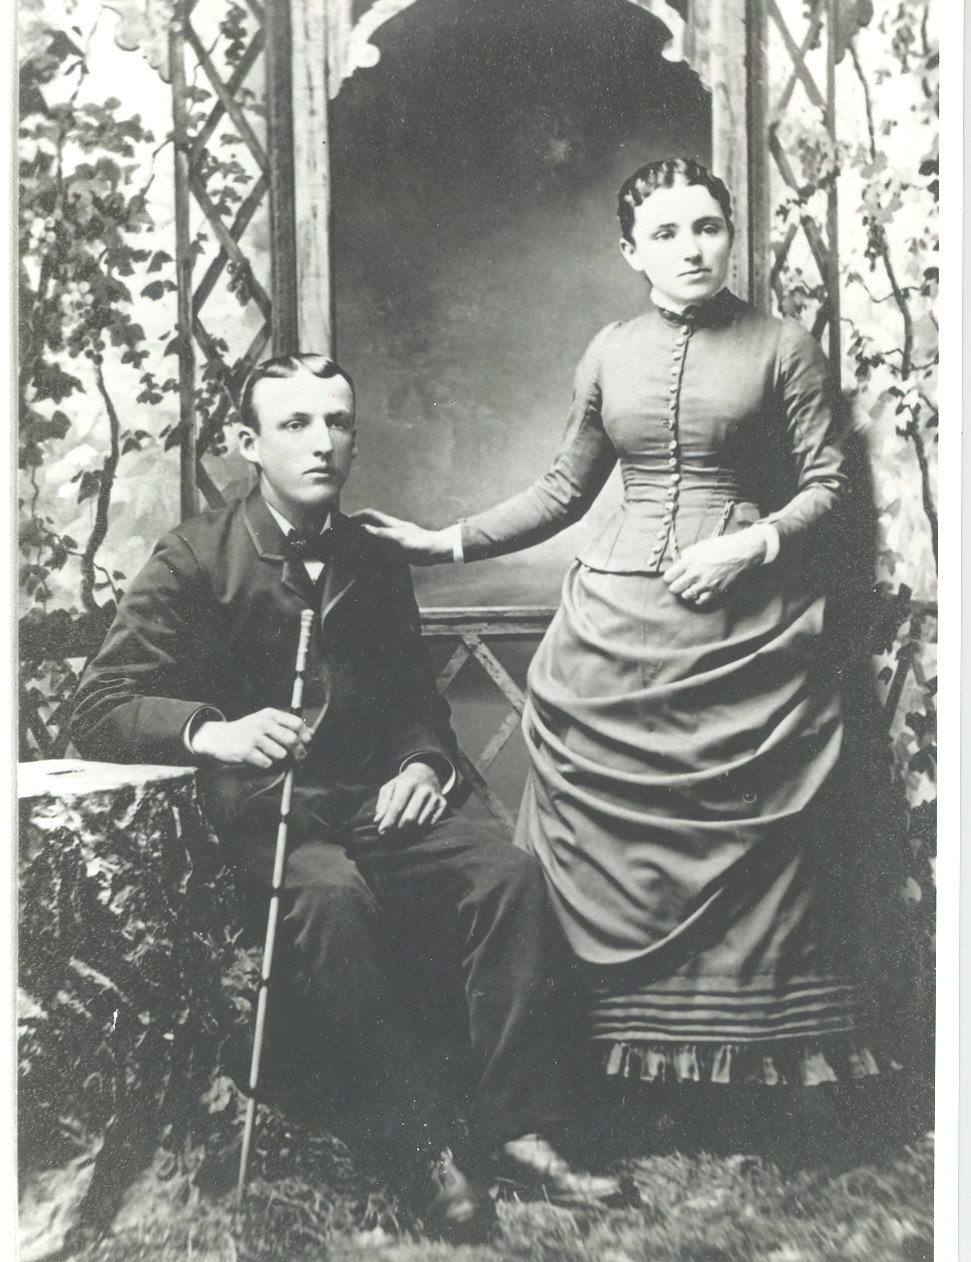
\includegraphics[height=0.35\textheight]{my_family/6.jpg}
\caption{\textit{left:} Jacob and Mary Hess. \textit{right:} Lois Spring 1974}
\end{figure}


Personality traits are more subjective.
What did I learn and what was I born with? From my mother I learned the power of a positive attitude.
My father may have dealt with some level of depression.
I've been aware of some in myself as well.

Both of my parents were hard workers who kept at the job until it was finished.
My mother was an extrovert and my father an introvert.
I come in the middle of that.
School was a positive experience for my mother and she stayed in until she completed 11th grade and her family could no longer support her.
My father completed eighth grade twice and ended his school years to become a farmer.
Both of my parents encouraged us to get an education.
School was a mixed bag for me.
Some aspects I enjoyed while others were difficult.
My mother was a reader and I followed that example.
Although I have clearly become my own unique person, my parents are present in the resources that have shaped who I am.




